\subsection{Seq2Seq model for machine conversation}
To construct a Seq2Seq model for machine conversation, we take similar setting as Google chatbot \cite{ncm}. The model is based on two LSTM layers: one for encoding and the other for decoding, as shown in the original paper of Seq2Sq2 model \cite{seq2seqO}. 

\begin{figure}[H]
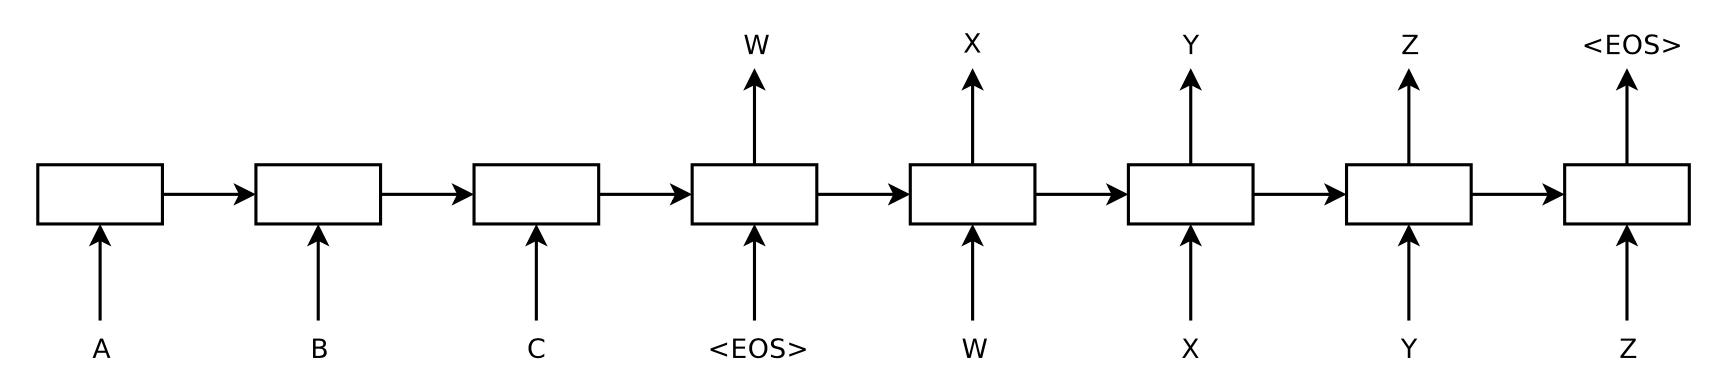
\includegraphics[width=0.4\textwidth]{seq2seq.png}
\caption{Illustration of Seq2Seq model. Figure is taken from the original paper \cite{seq2seqO}.}
\label{fig:seq2seq}
\end{figure}

The sentence is processed token by token, and the input sentence is read in reverse in LSTM, for introducing short-term dependencies in the data to make it easier for optimization \cite{seq2seqO}. The encoding part of the model (A, B, C in the figure) is for input sequence to encode the "thought" of input into a feature vector. The decoding part (W, X, Y, Z) is for generating a response from feature vector. Together we train the model end-to-end with gradient descent optimizer.

\subsection{Incorporating latent information unsupervised as the input to Seq2Seq model}
Applying the vanilla neural conversation model with seq2seq structure has various drawbacks, one of which appears as the respond might not be able to reflect the context, and inconsistency might occur across the conversation.

To solve the above-mentioned problem, we want to train a model that can encode the sentence not only precedes to our expected output, but also the context that the conversation occurs. We consider using Variational Recurrent Auto-Encoder \cite{vrae} that has been successfully applied in encoding the posterior distribution of time series data in \ref{fig:vrae}. The VRAE model shares the same re-parametrization with \cite{vae} while replaces the input and output to LSTM/RNN layers that can better capture the time dependencies.

\begin{figure*}[]
\centering
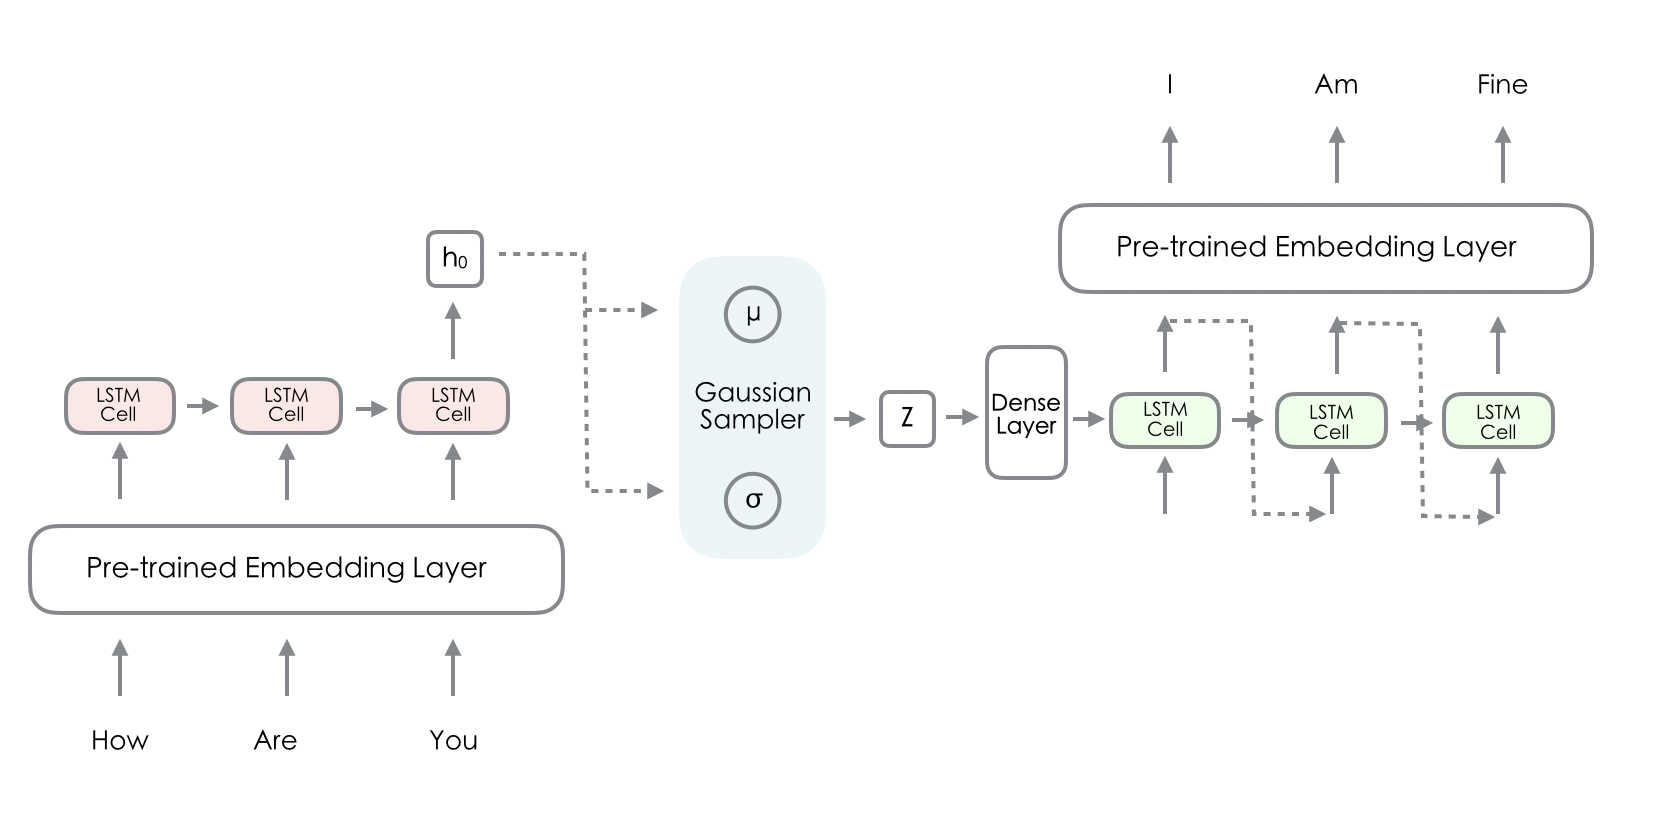
\includegraphics[width=0.8\textwidth]{VRAE.png}
\caption{Variational Recurrent Auto-encoder}
\label{fig:vrae}
\end{figure*}

VRAE can be trained as an independent model with sentences from the same resources of the seq2seq model for sentence prediction. It can be well regarded as another seq2seq model that automatically encodes the side information (context) that assists the core model to perform better predictions. While in the training process for neural conversation model, we use the pre-trained weight of the VRAE as a latent variable extractor, and with context information fed in, it produces the encoded information with which we can concatenate them in our core model, \ref{fig:proposed}.

\begin{figure*}[]
\centering
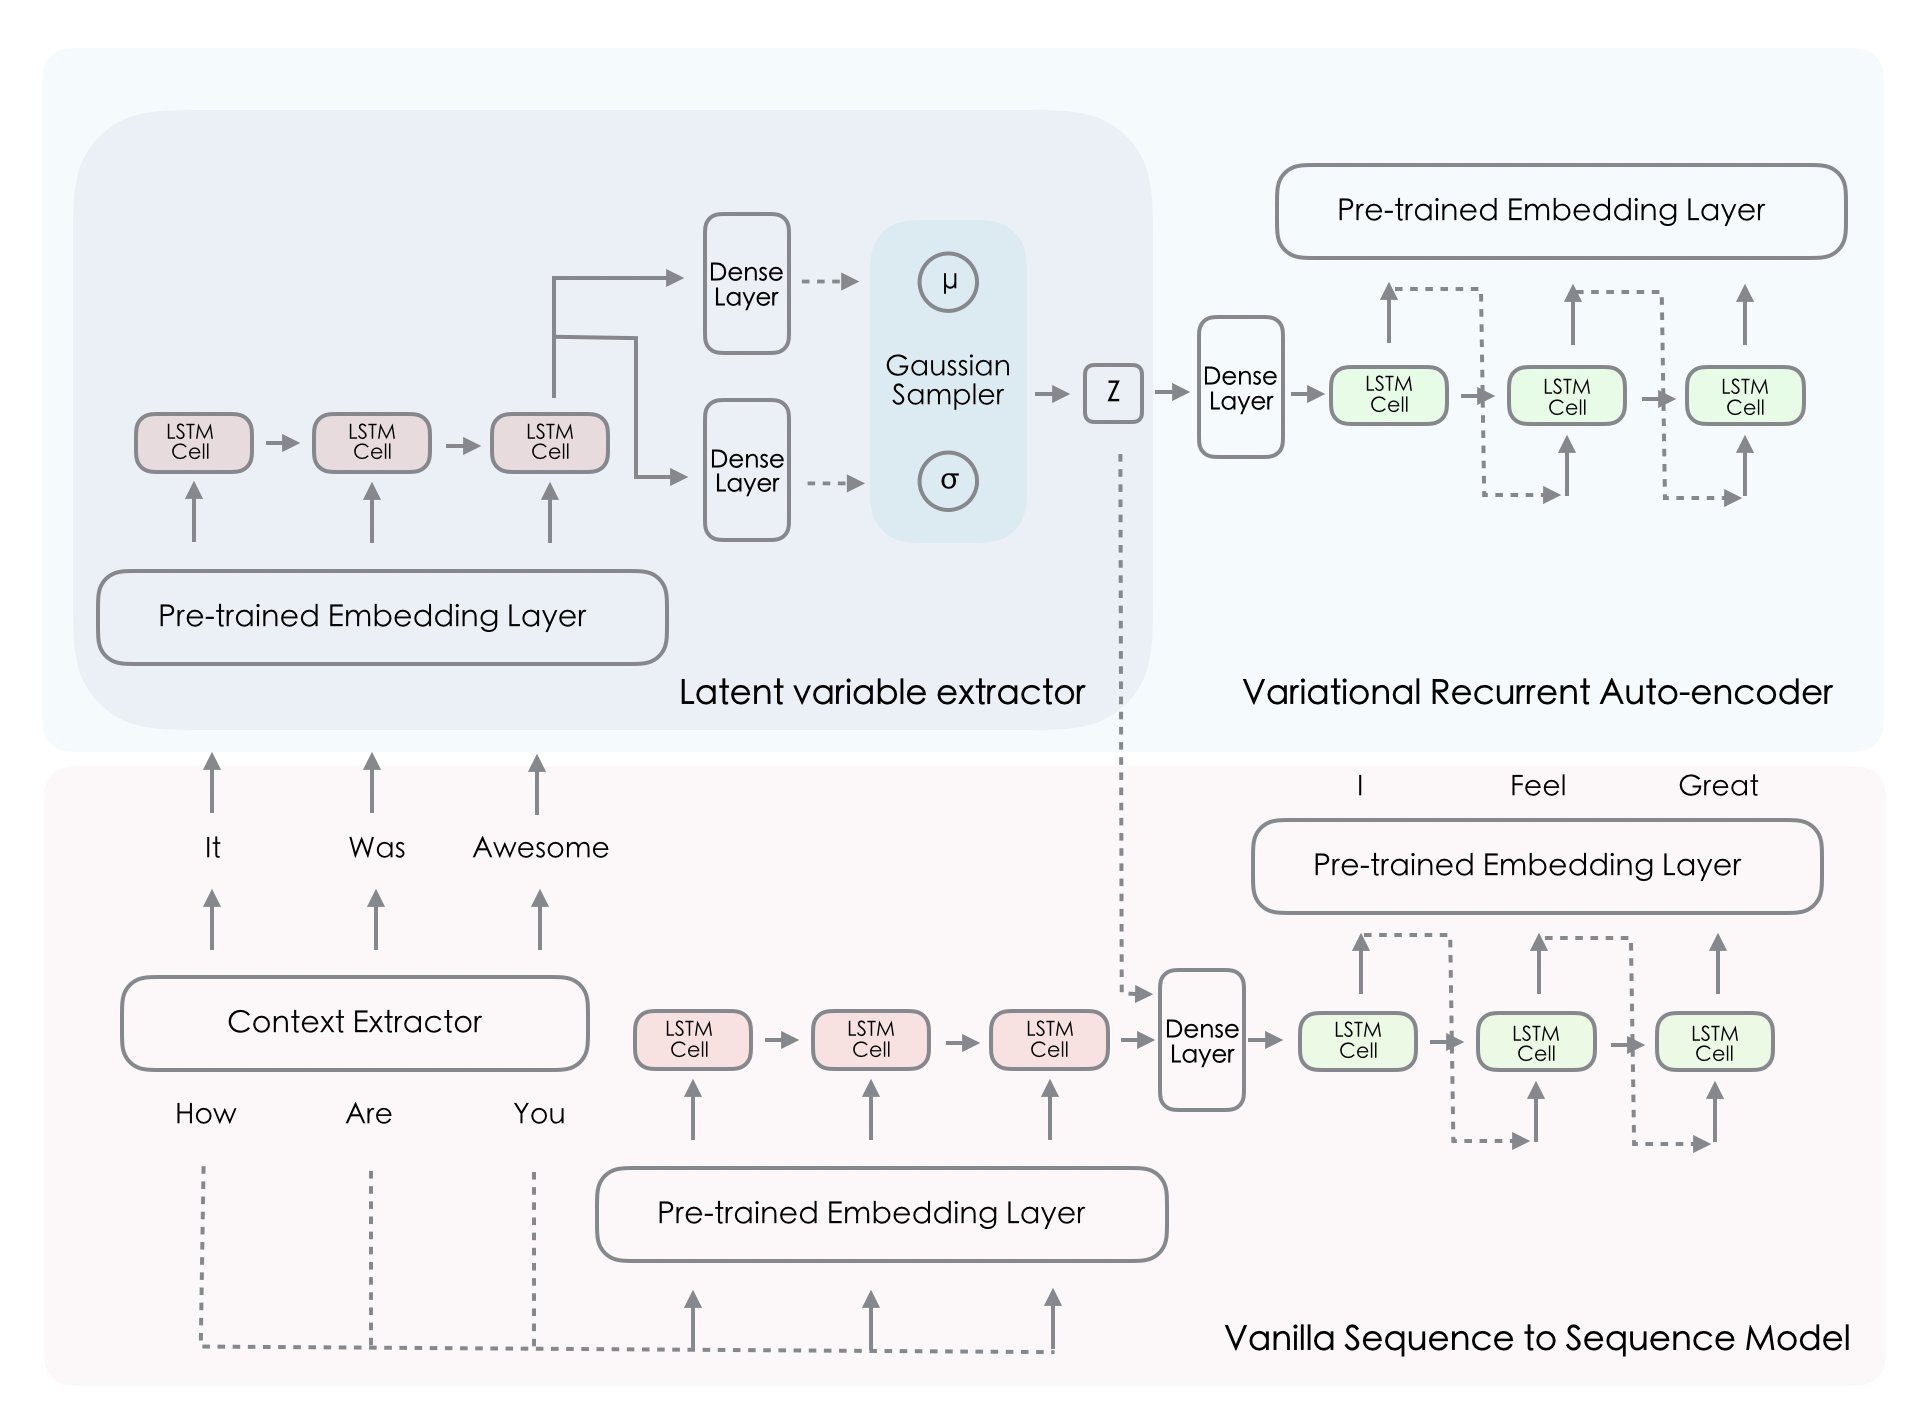
\includegraphics[width=0.8\textwidth]{proposed.png}
\caption{Proposed Method}
\label{fig:proposed}
\end{figure*}

\subsection{Incorporating latent variables in the training of Seq2Seq model}

Following the work in \cite{vnmt}, which introduces a variational model for neural machine translation that incorporates a continuous latent variable $z$ to model the underlying semantics of sentence pairs, we can also apply it to our neural conversation model that uses the same seq2seq model. 

We can also apply the method proposed by \cite{vrnn}, that explicitly models the dependencies between latent random variables across subsequent time steps.